\documentclass[letterpaper,11pt]{article}

% Palatino typeface for all text
\usepackage{tgpagella}

% Typesetting mathematics
\usepackage{eulervm}

% Remove hyphenation
\usepackage[none]{hyphenat}
% Maintain justification after removing hyphenation
\sloppy

% Crimson Text and fancy text stuff (like pasting unicode into your .tex file)
% \usepackage{crimson}
\usepackage[T1]{fontenc}
% \usepackage{fontspec}
\usepackage[utf8]{inputenc}
\usepackage[english]{babel}

% Customize page, text, section headings, and quotes
\usepackage[top=1in, bottom=1.5in, left=1.5in, right=1.5in]{geometry}
\usepackage{titlesec}
\usepackage{setspace}
\usepackage[begintext=``,vskip=\partopsep,leftmargin=0.5in,rightmargin=0.5in]{quoting}

% runin: make the abstract heading be part of the paragraph.
\usepackage[runin]{abstract}

% First, make footnotes flush w/ the bottom of the page even if there's some
% remnant whitespace. Second, I like my footnotes to be clickable to get to
% their original location in the text.
\usepackage[bottom]{footmisc}
\usepackage{footnotebackref}

\usepackage{graphicx}
\usepackage{xcolor}

% Caption requirements
\usepackage[
  tableposition=top,
  figureposition=bottom,
  labelfont=bf,
  labelsep=period,
  justification=centering,
]{caption}
\DeclareCaptionFont{8.5pt}{
    \fontsize{8.5pt}{14pt}\selectfont
    \spaceskip=1.0\fontdimen2\font plus 1.0\fontdimen3\font minus 1.0\fontdimen4\font
}
\captionsetup{font=8.5pt}

% Control space around table and figure captions
\captionsetup[figure]{aboveskip=8pt}
\captionsetup[figure]{belowskip=-17pt}
\captionsetup[table]{aboveskip=13pt}
\captionsetup[table]{belowskip=0pt}

% Customize tabular environment as per JDF 2.0
\let\oldtabular\tabular
\let\endoldtabular\endtabular
\renewenvironment{tabular}{
    \fontsize{8.5}{8.5}\selectfont
    \spaceskip=1.0\fontdimen2\font plus 1.0\fontdimen3\font minus 1.0\fontdimen4\font
    \oldtabular}{\endoldtabular}

% Custom space above and below \midrule horizontal line
\usepackage{booktabs}
\aboverulesep=0.5em
\belowrulesep=0.3em

\usepackage{float}      % better figures
\usepackage{enumitem}   % better lists
\usepackage{fancyhdr}   % better headers/footers
\usepackage{hyperref}   % better links

% Make math prettier
\usepackage{amsmath}
\usepackage{amssymb}

% Use APA citation format
\usepackage[natbibapa]{apacite}
\usepackage{natbib}
\setlength\bibhang{0.5in}

% Get the References section to be numbered as if it were created via \section
\usepackage[numbib]{tocbibind}


% Remove the comma between authors and years.
\AtBeginDocument{%
  \renewcommand{\BBAY}{}%% punctuation between authors and year
  % \renewcommand{\BBN}{: }%% punctuation between year and page number
  \renewcommand{\BBYY}{; }%% punctuation between multiple years
}

% Main body spacing
\setstretch{1.26}

% Abstract margins and style
\setlength{\absparindent}{0em}
\setlength{\absleftindent}{0.5in}
\setlength{\absrightindent}{0.5in}
\setlength{\abstitleskip}{-\absparindent}
\renewcommand{\abstracttextfont}{\normalfont}
\abslabeldelim{ \textemdash}
\renewcommand{\abstractnamefont}{\normalfont\bfseries\itshape}

% Paragraph indentation
\setlength{\parindent}{0pt}
\setlength{\parskip}{8.5pt}

% Level 1
\titleformat{\section}
  {\normalfont\fontsize{11}{0}\bfseries}
  {\thesection}{2pt}{\MakeUppercase}

% Level 2
\titleformat{\subsection}
  {\normalfont\fontsize{11}{0}\bfseries}
  {\thesubsection}{2pt}{}

% Level 3
\titleformat{\subsubsection}
  {\normalfont\fontsize{11}{0}\bfseries\itshape}
  {\textup{\thesubsubsection}}{2pt}{}

% Level 4 (The use of headings beyond Heading 3 is discouraged.)
\titleformat{\paragraph}[runin]
  {\normalfont\fontsize{11}{0}\bfseries\itshape}
  {\theparagraph}{2pt}{}

% Level 5 (Not specified in JDF 2.0)
% \titleformat{\subparagraph}
%   {\normalfont\fontsize{11}{0}\itshape}
%   {\theparagraph}{1em}{}

\titlespacing*{\section}{0pt}{7pt}{0pt}
\titlespacing*{\subsection}{0pt}{4.5pt}{0pt}
\titlespacing*{\subsubsection}{0pt}{4.5pt}{0pt}
\titlespacing*{\paragraph}{0pt}{4.5pt}{0pt}

% (Not specified in JDF 2.0)
% \titlespacing*{\subparagraph}{0pt}{8.5pt}{8.5pt}
% \titlespacing*{\subsubparagraph}{0pt}{8.5pt}{8.5pt}

% Just have the page number centered in footer.
\renewcommand{\headrulewidth}{0pt}
\setlength{\footskip}{0.5in}
\fancyhf{}
\cfoot{\thepage}
\pagestyle{fancy}

% Overwrite the title format, specifying font sizes and tightening space between
% the title text and the author.
%
% TODO: Make the spacing between lines a little bigger; things are too tight.
\makeatletter
\renewcommand{\maketitle}{\bgroup
   \begin{center}
   {\fontsize{17pt}{20}\selectfont \@title}
   \vspace{10pt}
   {\fontsize{11pt}{0}\selectfont \@author}
   \vspace{-11pt}
   \end{center}
}
\makeatother

% A pleasant blue to use for links.
\definecolor{ballblue}{HTML}{2ea3f2}

% Set a 0.5in margin for lists.
\setlist{leftmargin=0.5in}
\setlist{nolistsep}

% Increase interword spacing to match with JDF 2.0.
\spaceskip=1.5\fontdimen2\font plus 1.5\fontdimen3\font minus 1.5\fontdimen4\font

% Custom commands: superscript, subscript, and URL.
\newcommand{\super}[1]{$^{\text{#1}}$}
\newcommand{\subsc}[1]{$_{\text{#1}}$}
\newcommand{\link}[2]{\href{#1}{\underline{\smash{#2}}}}

% Custom \authoremail command that adds a clickable email
\newcommand{\authoremail}[2]{\author{#1\\\link{mailto:#2}{#2}}}

% Custom command for inline code-style
\usepackage{courier}
\usepackage{xcolor}
\definecolor{light-gray}{gray}{0.95}
\newcommand{\code}[1]{\colorbox{light-gray}{\texttt{#1}}}

% Sets up some nice PDF metadata
\hypersetup{
  pdftitle={},    % whatever your title is, or some shorter version
  pdfauthor={},   % your name, probably
  pdfsubject={},  % tags or a subject
  % bookmarks=true,
  % bookmarksopen=true,
  pdfpagemode=UseOutlines,
  colorlinks,
  citecolor=ballblue,
  urlcolor=ballblue,
  linkcolor=ballblue
}



\title{
  {{-cookiecutter.project_title_line_1-}} \\

  
    {{-cookiecutter.project_title_line_2-}} \\
  

  
    {{-cookiecutter.project_title_line_3-}} \\
  
  }

\authoremail{ {{-cookiecutter.author_name-}} }{ {{-cookiecutter.author_email-}} }

\begin{document}
\maketitle
\thispagestyle{fancy}

% You may include a new tex file here using:
% \input{<file_name>.tex}

\begin{abstract}%
If your paper requires an abstract, it should be placed at the top of the first page underneath the title block, preceded by the word \emph{Abstract} in bold italic. An extra 0.5'' should be added to both sides. Not all papers require abstracts; only those that would benefit from a high-level summary of the project or its background.
\end{abstract}

\section{Text}
Welcome to Joyner Document Format (JDF) 2.0! JDF is primarily intended to standardize page lengths while ensuring readability. Note that although you are required to use JDF for all written assignments, we will not perform explicit formatting checks. You should not worry too much about whether your submission conforms to every minute detail; the most important elements are margins, font, font sizes, and approximate line spacing. Use the paragraph styles built into this document. If you do so, you do not need to verify that the style was followed.

\huge\centerline{Handgloves}\normalsize

\begin{figure}[H]
  \centering
  
\includegraphics[scale=0.7]{figs/example-image1}
  \caption{Palatino. Make sure the live text (top) uses the same font as the image (bottom).}
  \label{fig::1}
\end{figure}

All text in JDF should be set in the Palatino typeface. It is available practically everywhere as a system font: Google Docs offers a version called \emph{Palatino Linotype}. It comes in regular and bold weights with matching italics.

\subsection{Body text}
Body text is set in the regular weight at 11 points with custom line spacing of 1.26, and 8.5 points of spacing added after each paragraph. It should be justified and paragraphs should not be indented. These styles can be automatically applied using the \emph{Normal} paragraph style.

\textbf{Bold} and \emph{italics} should be used for emphasis. Hyperlinks may be inserted in the text, as well as \texttt{in-line} code, superscripts \super{like this}, and subscripts \subsc{like this}.

\subsection{Title \& subtitle}
The paper title should be set in the regular weight at 17 points with 1.15 line spacing, centered at the top of the first page. The title may span up to three lines. For typical assignments, the document title may be as simple as “Assignment 1.” More specialized assignments may warrant more unique paper names, like “A Proposal to Create a New Document Format.”
The author’s name and email should come next unless you want to or were asked to submit anonymously, in which case this can be omitted. They should be set in the same size and weight as body text, centered. These styles can be applied using the Title and Subtitle paragraph styles.

\subsection{Headings}
Headings should all be set in the same size as body text (11 points) in bold. With the exception of \emph{Heading 1}, they should all have 8.5 points of space added before and after. They should be hierarchically numbered: Microsoft Word will do this automatically when you use the appropriate paragraph styles, but Google Docs users will need to number their headings manually.

\subsubsection{Heading 1}
Heading 1 should be set in all caps. It should have 11 points of space added before and 8.5 points of space added after.

\subsubsection{Headings 2-4}
Besides \emph{Heading 1}, which is set in caps, headings should always use sentence case (i.e., first word capitalized) rather than title case; after all, they are not titles. \emph{Heading 2} should be set in bold roman (upright), and \emph{Heading 3} should be set in bold italics. The use of headings beyond \emph{Heading 3} is discouraged.

\paragraph{Heading 4}
\emph{Heading 4} is provided as a run-in sidehead. Like \emph{Heading 3}, it is set in bold italics, but it should be followed by an em dash and flow right into the text, as seen at the beginning of the current paragraph. It should be used more as a list style than a heading style, e.g. to set off a list of principles in a heuristic evaluation.

\subsection{Page layout}
JDF uses the US Letter paper size (8.5'' x 11''). It has a top margin of 1'', and bottom and side margins of 1.5''. This yields a text block of 5.5'' x 8.5'', which is exactly $\frac{1}{2}$ the size of the page, divided lengthwise.

The page number should be included in the bottom margin, 1'' from the bottom of the page --- this creates symmetry with the top margin. No other elements should be placed in the margins.

\section{Presentational elements}
You are encouraged to use presentational elements liberally, as long as they add to the clarity of your submissions. They often require less space and fewer accompanying words to explain a given concept, and do a far better job of it.

\subsection{Figures}
Figures should always be centered on the page, although they may also take up the entire width and height of the text block. Figures should always be referenced in the text, and they should include a descriptive caption. Figures may also be equations, diagrams, or other kinds of content.

If your figure includes a white background (e.g. an interface design or graph), it may aid legibility to add a $\frac{1}{4}$ point black border.

\begin{figure}[H]
  \centering
  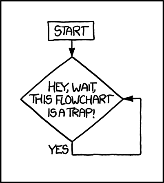
\includegraphics[scale=0.95]{figs/example-image2}
  \caption{Make sure your flowcharts are more useful than this one. Source: \link{https://xkcd.com/1195/}{XKCD}.}
  \label{fig::2}
\end{figure}

Figure captions should be centered beneath the corresponding figure. The label for the figure, e.g. “Figure 1,” should be bolded, and the entire caption should be 8.5 points with 14 points of line spacing. If need be, you may have one figure caption corresponding to multiple consecutive figures and use either locational descriptors (e.g. “top left,” “middle”) or labels (e.g. “A”, “B”) to map parts of the caption to parts of the figure. Make sure that caption falls on the same page as the corresponding figure or table; you may rearrange text to make this work.

\subsection{Tables}
You have freedom to format tables in the way that works best for your data. Generally, text should be left-aligned and numbers should be right-aligned or aligned at the decimal – you can do this using a \link{https://practicaltypography.com/tabs-and-tab-stops.html}{custom tab stop}. The default table style shown in \autoref{table:1} reduces the text size to be equal to the caption text.

Table captions should be formatted the same way as figure captions, but they should be placed above the table. The popular mnemonic for this is: figures at the foot, tables at the top. Like figures, tables should not exceed the margins and should be centered on the page.

\begin{table}[H]
  \centering
  \caption{Mathematical constants. Notice how the approximations align at the decimal.}
  \label{table:1}
  \begin{tabular}{@{}lcrl@{}}
    \textbf{Name} & \textbf{Symbol} & \textbf{Approximation} & \textbf{Description}\\
    \midrule
    Golden ratio & $\omega$ & 1.618 & Number such that the ratio of 1 to the number is equal\\
    & & & to the ratio of its reciprocal to 1\\
    \midrule
    Euler's number & $\epsilon$ & 2.71828 & Exponential growth constant\\
    \midrule
    Archimedes' & $\pi$ & 3.14 & The ratio between circumference and diameter of a\\
    constant & & & circle\\
    \midrule
    One hundred & A\super{+} & 100.00 & The grade we hope you'll all earn in this class
  \end{tabular}
\end{table}

\subsection{Additional elements}
There are additional elements you may want to include in your paper, such as in-line or block quotes, lists, and more. For other content types not covered here, you have reasonable flexibility in determining how it should be used in this format.

\subsubsection{Quotes}
If you would like to quote an outside source, you may do so with quotation marks followed by a citation. If a quote is fewer than three lines, you may write it in-line. It is acceptable to replace pronouns with their target in brackets for clarity. For example, “Heavy use of peer grading would compromise [the school’s] reputation” (Joyner, 2016). If a quote exceeds three lines, you should set it as its own paragraph with 0.5'' side margins, using the \emph{Blockquote} style.

\begin{quoting}
Whether or not the grades generated by peers are reliably similar to grades
generated by experts is only one factor worth considering, however. Student
perception is also an important factor. A recent study indicated that reliance
on peer grading is one of the top drivers of high MOOC dropout rates. This
problem may be addressed by reintroducing some expert grading where possible''
(Joyner 2016)
\end{quoting}

\subsubsection{Lists}
Bulleted and numbered lists are indented 0.5'' from the left margin, with the bullet or number hanging in the margin by 0.25'' (the default format).

\begin{itemize}
\item
  Here's an item.

\item
  Like numbered lists, the second line along a single line in a bulleted list is
  at the same level of indentation.
\end{itemize}

Bulleted lists follow the same format:
%
\begin{enumerate}
\item
  This is an item.
\item
  Note that the left side of the text is aligned, as are the numerals.
\item
  Notice also that a second line corresponding to the same bullet is also
  indented at the same level of the previous lines.
\end{enumerate}


\section{Procedural elements}

\notext

\subsection{In-line citations}
Articles or sources to which you refer should be cited in-line with the
authors' names and the year of publication.\footnote{In-line citations are preferred over footnotes, and we favor APA citation format for both in-line citations and reference lists. Refer to the \link{https://owl.purdue.edu/owl/research_and_citation/apa_style/apa_formatting_and_style_guide/in_text_citations_the_basics.html}{Purdue Online Writing Lab}, or follow the above examples. Footnotes should use 8.5 point text with 1.26 line spacing.
} The citation should be placed close
in the text to the actual claim, not merely at the end of the paragraph. For
example: students in the OMSCS program are older and more likely to be employed
than students in the on-campus program \citep{Joyner17}. In the event of
multiple authors, list them. For example: research finds sentiment analysis of
the text of OMSCS reviews corresponds to student-assigned ratings of the course
\citep{Newman18}. You may also cite multiple studies together. For example:
several studies have found students in the online version of an undergraduate
CS1 class performed equally with students in a traditional version
\citep{Joyner18a,Joyner18b,Joyner19}. If you would like to refer to an author in
text, you may also do so by including the year (in parentheses) after the
author's name in text. If a publication has more than 4 authors, you may list
only the first author followed by `et al' . For example:
Joyner~et~al.~(\citeyear{Joyner16}) claim that a round of peer review prior to
grading may improve graders' efficiency and the quality of feedback given. This
applies to parenthetical citations as well, e.g. \citep{Joyner16}.

\subsection{Reference lists}
References should be placed at the end of the paper in a dedicated section. Reference lists should be numbered and organized alphabetically by first author’s last name. If multiple papers have the same author(s) and year, you may append a letter to the end of the year to allow differentiated in-line text (e.g. Joyner, 2018a and Joyner, 2018b in the section above). If multiple papers have the same author(s), list them in chronological order starting with the older paper. Only works that are cited in-line should be included in the reference list. The reference list does not count against the length requirements.

\bibliographystyle{apacite}
\bibliography{references}



\clearpage
\section{Appendices}
You may optionally move certain information to appendices at the end of your paper, after the reference list. If you have multiple appendices, you should create a section with a Heading 1 of “Appendices.” Each appendix should begin with a descriptive Heading 2; appendices can thus be referenced in the body text using their heading number and description, e.g. “Appendix 5.1: Survey responses.” If you have only one appendix, you can label it with the word “Appendix” followed by a descriptive title, e.g., “Appendix: Survey responses.”

These appendices do not count against the page limit, but they should not contain any information required to answer the question in full. The body text should be sufficient to answer the question, and the appendices should be included only for you to reference or to give additional context. If you decide to move content to an appendix, be sure to summarize the content and note it in relevant place in the body text, e.g., “The raw data can be viewed in Appendix 5.1: Survey responses.”

\end{document}
